    \subsection{Opis}
    Architektura logiczna systemu składa się z trzech modułów, które współpracują ze sobą w celu zapewnienia 
    kompleksowej funkcjonalności systemu.

    \begin{itemize}
        \item \textbf{Konfigurator}
        \begin{itemize}
            \item Odpowiada za interakcję użytkownika z systemem poprzez interfejs graficzny. 
            Użytkownik ma możliwość dokonywania modyfikacji ustawień dotyczących działania oprogramowania
            wykonawczego za pomocą interfejsu.
            \item Umożliwia wprowadzanie ustawień takich jak kadrowanie obrazu, 
            edycja linii rysowanych na obrazie, wybór wykrywanych obiektów oraz parametryzacja 
            procesu wykrywania i informowania o obiektach.
        \end{itemize}
        
        \item \textbf{Dane konfiguracyjne}
        \begin{itemize}
            \item Stanowi pośrednią warstwę między konfiguratorem a oprogramowaniem wykonawczym. 
            Jest odpowiedzialny za przechowywanie ustawień konfiguracyjnych.
        \end{itemize}

        \item \textbf{Oprogramowanie wykonawcze}
        \begin{itemize}
            \item Jest odpowiedzialny za przetwarzanie obrazu z kamery 
            oraz realizację funkcji związanych z wykrywaniem i identyfikacją obiektów na drodze.
            \item Podczas działania oprogramowania wykonawczego, na ekranie wyświetlany jest 
            obraz z kamery lub nagranie wraz z elementami graficznymi, takimi jak linie i ostrzeżenia.
        \end{itemize}
    \end{itemize}
    

    \subsection{Schemat}
    \begin{figure}[H]
        \centering
        \resizebox{\columnwidth/2}{!}{%
        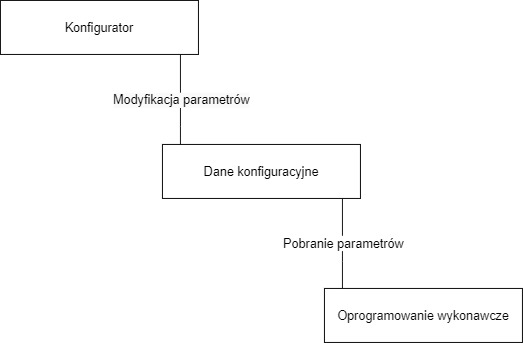
\includegraphics{Img/ISO42010_diagram.jpg}%
        }
        \caption{Schemat architektury logicznej systemu:}
        \label{fig:ISO42010_DIAGRAM}
    \end{figure}